% =====================================================================
%  Query rewriter: example simplifications, after [L14, s.8-9]
%  Compile:  pdflatex rewriter-examples.tex   (inside this folder)
%  Output:   rewriter-examples.pdf  -> 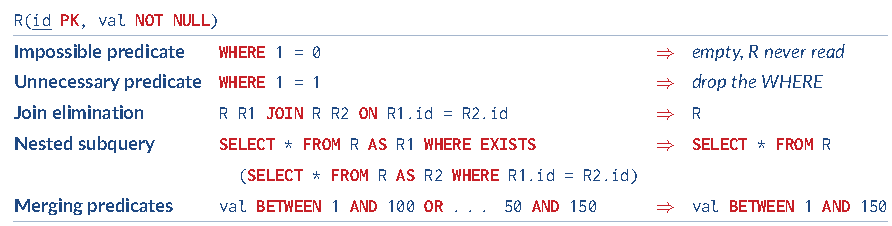
\includegraphics{rewriter-examples}
% =====================================================================
\makeatletter\def\input@path{{../../theme/}}\makeatother   % shared palette
\documentclass[border=2pt,11pt]{standalone}
\usepackage[T1]{fontenc}
\usepackage[defaultsans]{lato}
\usepackage[varqu,varl]{zi4}
\renewcommand{\familydefault}{\sfdefault}
\usepackage[table]{xcolor}
\usepackage{vinuni-palette}
\usepackage{array,amssymb}

\newcommand{\kw}[1]{\textcolor{vinuRed}{\textbf{#1}}}            % SQL keyword
\newcommand{\code}[1]{{\ttfamily\color{vinuNavy}\begin{tabular}[c]{@{}l@{}}#1\end{tabular}}}
\newcommand{\topic}[2]{\textbf{#1}\par{\scriptsize\color{vinuRed}#2}}
\newcommand{\goesto}{\textcolor{vinuRed}{\large$\Rightarrow$}}

\begin{document}
\color{vinuNavy}\footnotesize
\setlength{\tabcolsep}{5pt}
\renewcommand{\arraystretch}{1.08}
\begin{tabular}{@{}>{\raggedright\arraybackslash}m{36mm} l c l@{}}
  \multicolumn{4}{@{}l@{}}{\colorbox{vinuNavy!8}{\ttfamily\kw{CREATE TABLE} R ( id \kw{INT PRIMARY KEY}, val \kw{INT NOT NULL} )}}\\[2pt]
  \arrayrulecolor{vinuNavy!40}\hline
  \rowcolor{white}
  \topic{Impossible predicate}{} &
    \code{\kw{SELECT} * \kw{FROM} R \kw{WHERE} 1 = 0} & \goesto &
    \code{\sffamily\itshape empty result (R is never read)} \\
  \rowcolor{vinuLightGray}
  \topic{Unnecessary predicate}{} &
    \code{\kw{SELECT} * \kw{FROM} R \kw{WHERE} 1 = 1} & \goesto &
    \code{\kw{SELECT} * \kw{FROM} R} \\
  \rowcolor{white}
  \topic{Join elimination}{needs: id is a PK (unique \& not null)} &
    \code{\kw{SELECT} R1.*\\ \ \ \kw{FROM} R \kw{AS} R1 \kw{JOIN} R \kw{AS} R2\\ \ \ \ \ \kw{ON} R1.id = R2.id} & \goesto &
    \code{\kw{SELECT} * \kw{FROM} R} \\
  \rowcolor{vinuLightGray}
  \topic{Ignoring a nested subquery}{needs: id is not null} &
    \code{\kw{SELECT} * \kw{FROM} R \kw{AS} R1\\ \ \kw{WHERE EXISTS} (\kw{SELECT} * \kw{FROM} R \kw{AS} R2\\ \ \ \ \ \ \ \ \ \ \ \ \ \ \ \kw{WHERE} R1.id = R2.id)} & \goesto &
    \code{\kw{SELECT} * \kw{FROM} R} \\
  \rowcolor{white}
  \topic{Merging predicates}{[1,100] $\cup$ [50,150] = [1,150]} &
    \code{\kw{SELECT} * \kw{FROM} R\\ \ \kw{WHERE} val \kw{BETWEEN} 1 \kw{AND} 100\\ \ \ \ \ \kw{OR} val \kw{BETWEEN} 50 \kw{AND} 150} & \goesto &
    \code{\kw{SELECT} * \kw{FROM} R\\ \ \kw{WHERE} val \kw{BETWEEN} 1 \kw{AND} 150} \\
  \hline
\end{tabular}
\end{document}
